% Faithful native paths from source/普通高考/2009/2009辽宁理.pdf, page 1.
% Original outlines, connected rock fissures, solid/dashed edges and shaded regions retained.
% Labels retain their original objects; no arbitrary geometric substitute or raster wrapper.
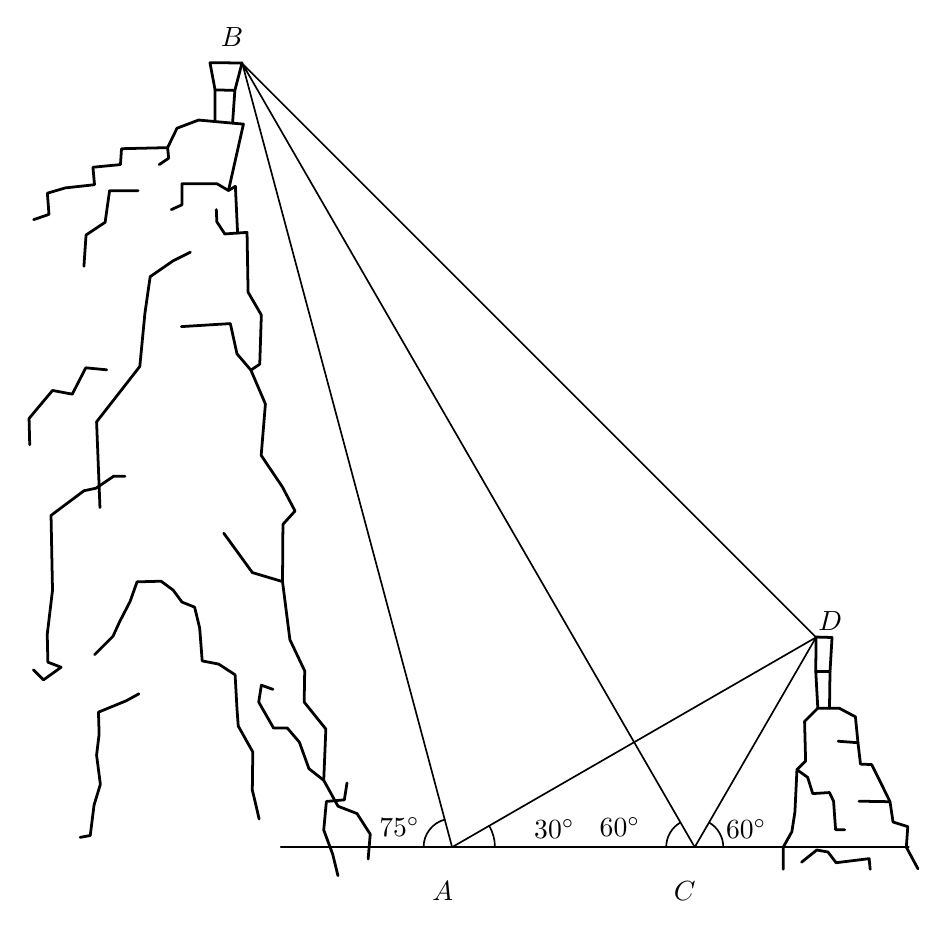
\begin{tikzpicture}[x=1cm,y=1cm,font=\normalsize,line join=round,line cap=round]
\path[draw=black,line width=0.6pt] (3.70186,1.12005) -- (11.67696,1.12005) ;
\path[draw=black,line width=0.6pt] (5.87689,1.12005) -- (3.21246,11.07080) -- (10.49879,3.78448) -- (8.95814,1.12005) -- (3.21246,11.07080) ;
\path[draw=black,line width=0.6pt] (10.49883,3.78446) -- (5.87691,1.12004) ;
\path[draw=black,line width=1.0pt] (1.15267,1.24421) -- (1.28119,1.26831) -- (1.32940,1.65387) -- (1.40971,1.91898) -- (1.36156,2.28849) -- (1.39366,2.55359) -- (1.38561,2.83467) -- (1.73907,2.97931) -- (1.89969,3.06768) ;
\path[draw=black,line width=1.0pt] (3.42599,1.47715) -- (3.37778,1.68599) -- (3.33935,1.84508) -- (3.34561,2.32866) -- (3.16089,2.65802) -- (3.14484,2.87490) -- (3.12074,3.30868) -- (2.91190,3.44520) -- (2.70300,3.48535) -- (2.67084,3.90307) -- (2.60665,4.16817) -- (2.44596,4.23244) -- (2.33349,4.38506) -- (2.18086,4.49754) -- (1.87561,4.48947) -- (1.78724,4.24049) -- (1.65072,3.97539) -- (1.57035,3.79866) -- (1.33741,3.56573) ;
\path[draw=black,line width=1.0pt] (0.55824,3.37290) -- (0.68676,3.24437) -- (0.91164,3.40506) -- (0.74296,3.46932) -- (0.73497,3.82273) -- (0.80180,4.38259) -- (0.78312,5.33295) -- (1.20085,5.64619) -- (1.35347,5.67835) -- (1.57842,5.83098) -- (1.72299,5.83098) ;
\path[draw=black,line width=1.0pt] (0.51259,6.23005) -- (0.50403,6.56459) -- (0.80179,6.92010) -- (1.05295,6.87329) -- (1.22444,7.20784) -- (1.49037,7.18206) ;
\path[draw=black,line width=1.0pt] (1.40454,5.43242) -- (1.36170,6.52166) -- (1.91057,7.22494) -- (1.97521,7.89786) -- (2.04197,8.36489) -- (2.33105,8.56503) -- (2.55344,8.67621) ;
\path[draw=black,line width=1.0pt] (4.42686,0.75755) -- (4.36049,1.02936) -- (4.24641,1.33814) -- (4.27999,1.70055) -- (4.50819,1.72076) -- (4.54176,1.93554) ;
\path[draw=black,line width=1.0pt] (4.81024,0.96894) -- (4.83710,1.28442) -- (4.66925,1.54619) -- (4.42761,1.64019) -- (4.24641,1.96904) -- (4.05849,2.11674) -- (3.93764,2.45236) -- (3.78329,2.63358) -- (3.60872,2.63358) -- (3.42080,2.96249) -- (3.45438,3.17726) -- (3.60201,3.12355) ;
\path[draw=black,line width=1.0pt] (4.24640,1.96906) -- (4.27326,2.62018) -- (3.99805,2.96251) -- (4.00476,3.35850) -- (3.81684,3.75455) -- (3.72285,4.49287) -- (3.34023,4.60695) -- (2.97685,5.10761) ;
\path[draw=black,line width=1.0pt] (3.72285,4.49289) -- (3.72835,5.22009) -- (3.88194,5.38902) -- (3.72069,5.69614) -- (3.45194,6.09545) -- (3.50571,6.74809) -- (3.32144,7.17810) -- (3.14482,7.38539) -- (3.06036,7.76929) -- (2.43841,7.73092) ;
\path[draw=black,line width=1.0pt] (1.20087,8.49725) -- (1.22780,8.89408) -- (1.46988,9.05546) -- (1.52685,9.45765) -- (1.88932,9.45765) ;
\path[draw=black,line width=1.0pt] (3.32141,7.17808) -- (3.43376,7.25301) -- (3.45396,7.87849) -- (3.28580,8.16769) -- (3.27238,8.92770) -- (2.98988,8.90749) -- (2.88899,9.06222) -- (2.88228,9.21690) ;
\path[draw=black,line width=1.0pt] (3.15240,8.91910) -- (3.12440,9.51280) -- (3.03699,9.45903) -- (2.88904,9.54644) -- (2.44516,9.54644) -- (2.44516,9.27744) -- (2.31062,9.21687) ;
\path[draw=black,line width=1.0pt] (0.56195,9.08909) -- (0.75696,9.15635) -- (0.73682,9.42535) -- (0.96547,9.49261) -- (1.33537,9.53296) -- (1.31524,9.75490) -- (1.66492,9.78854) -- (1.67843,9.99034) -- (2.26354,10.00376) -- (2.27698,9.86923) -- (2.15594,9.78854) ;
\path[draw=black,line width=1.0pt] (2.26354,10.00377) -- (2.38324,10.25059) -- (2.65696,10.35418) -- (3.22661,10.30239) -- (3.03696,9.45900) ;
\path[draw=black,line width=1.0pt] (3.20841,11.07894) -- (3.11781,10.73046) -- (2.86626,10.73762) -- (2.80162,11.08253) -- cycle ;
\path[draw=black,line width=1.0pt] (2.86630,10.73766) -- (2.86501,10.33527) ;
\path[draw=black,line width=1.0pt] (3.11777,10.73046) -- (3.08849,10.31498) ;
\path[draw=black,line width=1.0pt] (10.31442,0.92893) -- (10.50811,1.08385) -- (10.65019,1.05809) -- (10.75351,0.92246) -- (11.17316,0.97413) -- (11.18607,0.83851) ;
\path[draw=black,line width=1.0pt] (10.08200,0.83854) -- (10.08200,1.12006) -- (10.19180,1.31630) -- (10.23048,1.56810) -- (10.25630,2.10399) -- (10.39193,2.00712) -- (10.45651,1.80052) -- (10.66956,1.81344) -- (10.72116,1.70373) -- (10.74699,1.34214) -- (10.86324,1.34214) ;
\path[draw=black,line width=1.0pt] (11.79298,0.84498) -- (11.64540,1.12005) -- (11.66381,1.38086) -- (11.47659,1.43899) -- (11.43785,1.69725) -- (11.04402,1.70370) ;
\path[draw=black,line width=1.0pt] (11.43785,1.69722) -- (11.32161,1.93611) -- (11.20542,2.16852) -- (11.06335,2.17499) -- (11.03112,2.44616) -- (10.77926,2.46554) ;
\path[draw=black,line width=1.0pt] (10.25633,2.10396) -- (10.36611,2.21375) -- (10.35320,2.71735) -- (10.52105,2.88520) -- (10.79221,2.88520) -- (10.99881,2.77548) -- (11.03110,2.44617) ;
\path[draw=black,line width=1.0pt] (10.52106,2.88520) -- (10.49522,3.35011) -- (10.67599,3.35011) -- (10.66954,2.88520) ;
\path[draw=black,line width=1.0pt] (10.49522,3.35009) -- (10.49881,3.78852) -- (10.70181,3.78265) -- (10.67599,3.35009) ;
\path[draw=black,line width=0.6pt] (8.59566,1.12005) .. controls (8.59566,1.24954) and (8.66479,1.36923) .. (8.77694,1.43400) ;
\path[draw=black,line width=0.6pt] (5.51439,1.12005) .. controls (5.51439,1.28413) and (5.62462,1.42774) .. (5.78306,1.47019) ;
\path[draw=black,line width=0.6pt] (9.32069,1.12005) .. controls (9.32069,1.24954) and (9.25156,1.36923) .. (9.13942,1.43400) ;
\path[draw=black,line width=0.6pt] (6.42064,1.12005) .. controls (6.42064,1.21545) and (6.39551,1.30931) .. (6.34781,1.39193) ;
\node[anchor=base west,inner sep=0pt,outer sep=0pt] at (5.62514,0.44478) {$A$};
\node[anchor=base west,inner sep=0pt,outer sep=0pt] at (2.94102,11.28737) {$B$};
\node[anchor=base west,inner sep=0pt,outer sep=0pt] at (8.69425,0.44478) {$C$};
\node[anchor=base west,inner sep=0pt,outer sep=0pt] at (10.52686,3.87041) {$D$};
\node[anchor=base west,inner sep=0pt,outer sep=0pt] at (4.95223,1.25701) {$75^{\circ}$};
\node[anchor=base west,inner sep=0pt,outer sep=0pt] at (6.91931,1.22504) {$30^{\circ}$};
\node[anchor=base west,inner sep=0pt,outer sep=0pt] at (7.75105,1.25701) {$60^{\circ}$};
\node[anchor=base west,inner sep=0pt,outer sep=0pt] at (9.35565,1.22504) {$60^{\circ}$};
\end{tikzpicture}
